\input{../YKY-preamble.tex}
\setmainfont[BoldFont=Alibaba_Sans_Regular.otf,ItalicFont=Alibaba_Sans_Light_Italic.otf]{Alibaba_Sans_Light.otf}
	
\usepackage[active,tightpage]{preview}		% for continuous page(s)
\renewcommand{\PreviewBorder}{0.5cm}
\renewcommand{\thempfootnote}{\arabic{mpfootnote}}

\usepackage[absolute,overlay]{textpos}		% for page number on upper left corner

\usepackage{color}
\usepackage{mathtools}
\usepackage[hyperfootnotes=false]{hyperref}

% \usepackage[backend=biber,style=numeric]{biblatex}
% \bibliography{../AGI-book}
% \renewcommand*{\bibfont}{\footnotesize}

\usetikzlibrary{shapes}
\usepackage[export]{adjustbox}				% ??
\usepackage{verbatim} % for comments
% \usepackage{newtxtext,newtxmath}	% Times New Roman font

\titleformat{\subsection}[hang]{\bfseries\large\color{blue}}{}{0pt}{} 
% \numberwithin{equation}{subsection}

\newcommand{\underdash}[1]{%
	\tikz[baseline=(toUnderline.base)]{
		\node[inner sep=1pt,outer sep=10pt] (toUnderline) {#1};
		\draw[dashed] ([yshift=-0pt]toUnderline.south west) -- ([yshift=-0pt]toUnderline.south east);
	}%
}%


%\DeclareSymbolFont{symbolsC}{U}{txsyc}{m}{n}
%\DeclareMathSymbol{\strictif}{\mathrel}{symbolsC}{74}
\DeclareSymbolFont{AMSb}{U}{msb}{m}{n}
\DeclareSymbolFontAlphabet{\mathbb}{AMSb}
% \setmathfont{Latin Modern Math}
\DeclareMathOperator*{\argmin}{arg\,min}

% \usepackage[most]{tcolorbox}
\tcbset{on line, 
	boxsep=4pt, left=0pt,right=0pt,top=0pt,bottom=0pt,
	colframe=red,colback=pink,
	highlight math style={enhanced}
}
\newcommand{\atom}{\vcenter{\hbox{\tcbox{....}}}}

\let\oldtextbf\textbf
\renewcommand{\textbf}[1]{\textcolor{blue}{\oldtextbf{#1}}}

\newcommand{\logic}[1]{{\color{violet}{\textit{#1}}}}
\newcommand{\underconst}{\includegraphics[scale=0.5]{../2020/UnderConst.png}}
\newcommand{\KBsymbol}{\vcenter{\hbox{\includegraphics[scale=1]{../KB-symbol.png}}}}
\newcommand{\token}{\vcenter{\hbox{
\includegraphics[scale=1]{token.png}}}}
\newcommand{\proposition}{\vcenter{\hbox{
\includegraphics[scale=0.8]{proposition.png}}}}

\begin{document}

\begin{preview}

\cc{
\title{\vspace{-1.5cm} \bfseries\color{blue}{\LARGE Transformer 完全符合逻辑结构}}
}{
\title{\vspace{-1.5cm} \bfseries\color{blue}{\LARGE Transformer Has Full Logic Structure}}
}

% \author{YKY} % Your name
\date{\vspace{-2cm}} % Date, can be changed to a custom date

\maketitle

\setcounter{section}{-1}

% (1) Circled page number on upper left corner
\begin{textblock*}{5cm}(2.1cm,2.3cm) % {block width} (coords) 
{\color{red}{\large \textcircled{\small 1}}}
\end{textblock*}

\begin{minipage}{\textwidth}
\setlength{\parskip}{0.4\baselineskip}

承上文: 我提出了用逻辑结构加速 Transformer 的方法,但详细分析之后,竟然发现 Transformer 跟逻辑结构是完全重合的! 这结果有点令我失望(因为我一直以为自己能「魔改」Transformer 并且胜过它),但其实是非常正面的结果,也加深了我们对 Transformer 和逻辑结构的认识。

以下 讲述我思考 ``logic Transformer'' 的细节:

逻辑有「双层结构」: \uline{命题由概念原子构成,命题是可交换的,而概念不可交换}。 

逻辑系统的 \textbf{状态} 是一堆命题的集合,也就是 ``sequence of sequences'' 的结构。 

%这个 双层结构 可以用以下这种「魔改」的 Transformer 处理:
%\begin{equation}
%\vcenter{\hbox{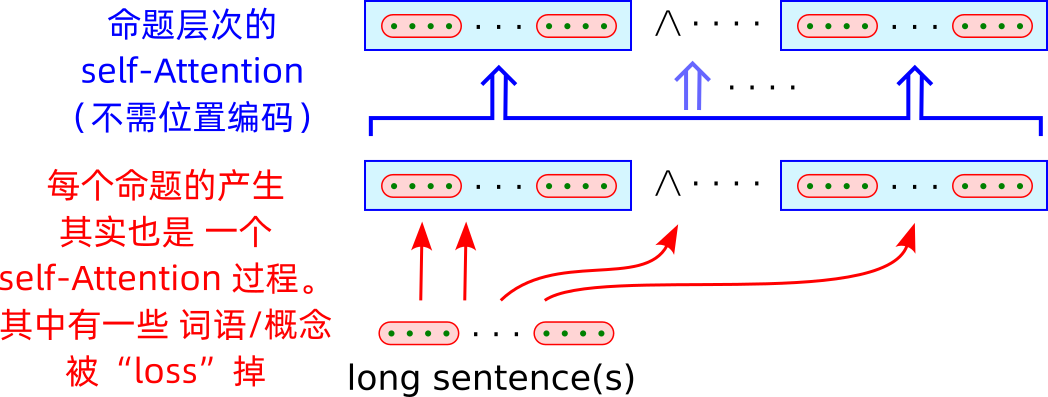
\includegraphics[scale=1]{seq-to-seq-seq-with-Transformer.png}}}
%\end{equation}

\subsection{命题内部层次 (sub-propositional level)}

第一层 ``lossy Self-Attention'' 将一个 长句子 分拆成 $n$ 个命题,命题可以由数量不同的 概念表示。 

例如,句子「拜登 2月 在白宫 就中美贸易问题发言」可以分拆为:
\begin{itemize}
	\item 「拜登在白宫」
	\item 「拜登发言」
	\item 「发言关于中美贸易问题」
	\item 「发言发生在2月」
\end{itemize}
等 几个 \textbf{较短的} 命题。 $n$ 的数目 视乎 句子复杂的程度而定。

\color{teal}
我初时提出,每个 短命题 可以用一个 ``lossy Self-Attention'' 产生:(输出的 tokens 数目比输入少)
\begin{equation}
\vcenter{\hbox{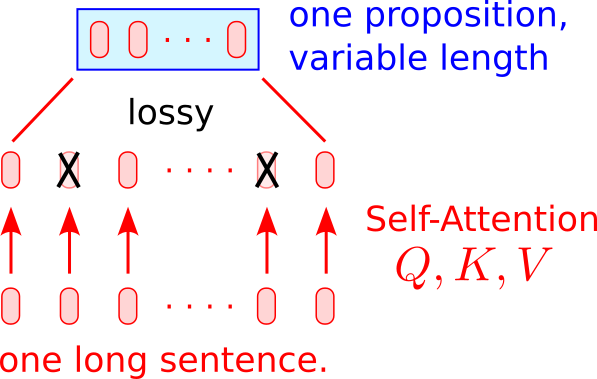
\includegraphics[scale=1]{Self-Attention_lossy.png}}}
\end{equation}
但这里出了问题: lossy 的意思是 将某些 输入的 tokens 省略掉,但这个动作是 \oldtextbf{不可微}的,因为它改变了 向量的维数,而维数是 拓扑不变量,意思是说: 任何(可逆的)连续映射不能改变空间的维数,而可微函数只是连续映射的一个特例。 除非放弃可逆性,那就表示 两个不同的自然语言句子 有可能映射到同一个命题。 \color{black}

我们需要的映射是: sequence $\rightarrow$ shorter sequence.  例如,由 10个 tokens 变成 3个 tokens:
\begin{equation}
\overbrace{\mbox{tok} \times \mbox{tok} \times ... \times \mbox{tok}}^{\mbox{10 times}} \rightarrow \mbox{tok} \times \mbox{tok} \times \mbox{tok}
\end{equation}
这两边的维数肯定是不同的,所以 injectiveness 必须放弃。 也就是说,两个不同的长序列 有可能映射到同一个短序列\footnote{这说法有点不准确: 因为深度学习用了所谓 ``embedding'',例如 \textbf{Word2vec} ,这种嵌入的「维数」没有良好定义。 在计算机上实践时,我们惯用 维数 = 512,但那是可以改变的。 那么我们也可以改变 embedding 的维数,将多个 tokens 挤进较小的空间里,也是可以的,但似乎比较麻烦。 厘清这种 embedding 的数学意义(它是不是有向量空间结构?微分流型结构?连续性跟离散的符号有何关系?),是一个很重要的问题,日后再谈.... }。

有个简单的解决办法是: 将自然语言句子映射到 一个长度\textbf{固定}的向量,它的内容是几个意思的\textbf{叠加}(图左):
\begin{equation}
\label{fig:fixed-width-Self-Attention}
\vcenter{\hbox{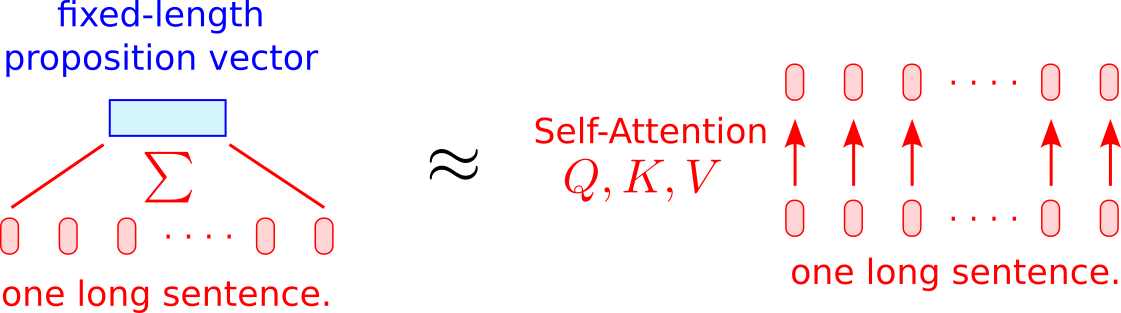
\includegraphics[scale=1]{Self-Attention_fixed_width.png}}}
\end{equation}
但传统 Transformer 的做法 就是这种做法的一个特例! Dot product similiarity 乘以每个 token 的 $V$ 值,然后 \textbf{相加} 得到输出。 这就是一种 \uline{将概念叠加的逻辑命题}。 换句话说,输出的 $\token$ 是一个 $\proposition$。 这很合理,因为在逻辑里,可交换的东西就是命题(若命题是真的,枚举它们的次序不重要),而 Self-Attention 的特点就是 equivariance.

但概念的叠加 丧失了 \textbf{不可交换性}: 我爱你 = 你爱我,世界没有失恋。 但似乎可以绕过这问题: 例如「我爱你」可以分拆为三个子命题:
\begin{itemize}
	\item 爱 = 动词
	\item 我 = 主语
	\item 你 = 宾语
\end{itemize}
这样分拆之后,命题内部不再需要次序(也就是可交换的)。 这是一种特殊的逻辑语法,看来未尝不可。

将以上 (\ref{fig:fixed-width-Self-Attention}) 的结构 横向重复 $n$ 次:(简单起见,$(Q,K,V)$ 简写为 $QKV$)
\begin{equation}
\vcenter{\hbox{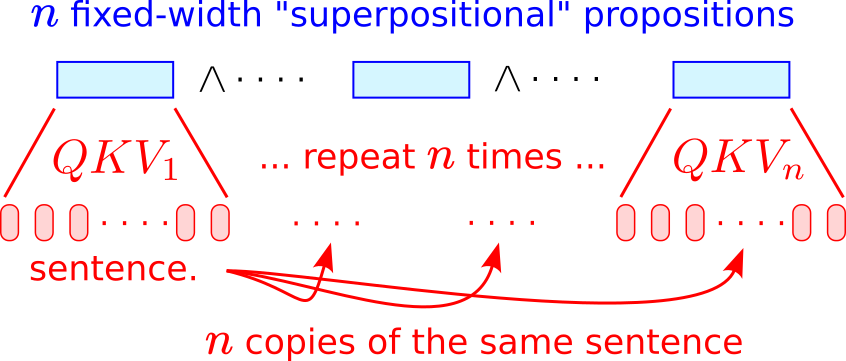
\includegraphics[scale=1]{Self-Attention_repeated.png}}}
\end{equation}
如果每个 $QKV_i$ 都是一样的,那就是传统的 Transformer 结构; 如果每个 $QKV_i$ 不同,那就对应于 \textbf{Multi-Head Attention}. 

以前说过,每个 $QKV_i$ 可以看成是一个 rule base,它们是独立运作的。 Multi-Head Attention 相当于说,同一堆前提可以推出不同的结论,即
\begin{equation}
	A \wedge B \wedge C \wedge ... \rightarrow X \mbox{ or } Y
\end{equation}
这导致逻辑推论可能出现分歧,这种分歧似乎没有太大效益,因为我曾听说 Multi-Head Attention 的功效并不显著。 在 Prolog 语言里也没有这种 ``or'' 语法,但 Prolog 作为编程语言还是 OK 的。

% 又或者可以看成 将很多层的 Transformer layers 水平地摊开来,\textbf{将深度变成广度}。 我推测这是没有问题的,因为 强化学习的「无限 loop」跟 深度的效果一样。

\subsection{命题层次 (Propositional level)}

第二层 我称为 ``symmetric Self-Attention'',它比较简单,而且\textbf{不需要 位置编码}:
\begin{equation}
\vcenter{\hbox{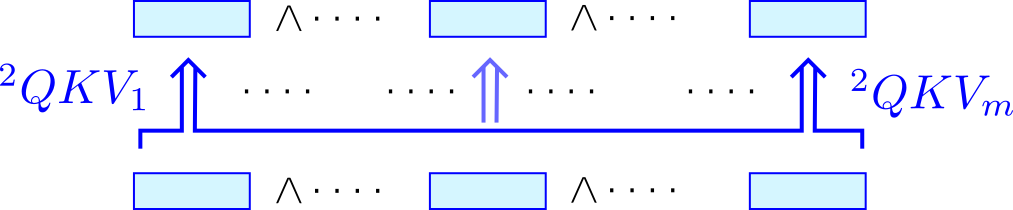
\includegraphics[scale=1]{Self-Attention_symmetric.png}}}
\end{equation}
其实在 传统的多层 Transformer 里面,除了第一层也没有位置编码。 这也表示,传统 Transformer 跟 逻辑结构 完全重合。

\end{minipage}
\end{preview}

\begin{preview}
\begin{minipage}{\textwidth}
\setlength{\parskip}{0.4\baselineskip}

\begin{textblock*}{20cm}(2.1cm,2cm) % {block width} (coords) 
	{\color{red}{\large \textcircled{\small 2}}}
	\hspace{8cm}
	\color{blue}{\footnotesize \cc{逻辑 Transformer}{Logic Transformer}}
\end{textblock*}
\vspace*{0.3cm} 

\end{minipage}
\end{preview}
\end{document}
